\chapter{Reducción de datos con IRAF}
En esta clase abordaremos el procedimiento estándar para combinar imágenes y crear archivos master. Los datos que usaremos son los de un sistema binario de una estrella de neutrones y una estrella normal. Dicha clase de sistemas se conoce como <<\emph{viuda negra}>>. Los datos se encuentran en este enlace: \url{https://drive.google.com/drive/folders/1TxopD_fIa1ZHplm_SH0Gvhe663psuJn-?usp=sharing}.

\section{Combinando imágenes}
Para realizar las tareas de combinación de imágenes, necesitaremos utilizar la terminal de comandos junto con la interfaz de pyraf y movernos a través de los directorios de manera recurrente. Para representar la terminal de IRAF se utilizarán los caracteres <<\norbash{-->}>>, como en el siguiente ejemplo:

\begin{shell}
--> 
\end{shell}

Ten en cuenta que para utilizar algunos comandos de GNU/Linux dentro de la interfaz de Pyraf, se necesita anteponer el símbolo <<\norbash{!}>> a cada comando. Recuerda esto al momento de seguir los pasos durante toda esta clase. 

\subsection{Creando un archivo master bias}
Para crear un archivo master bias, primero dirígete a la carpeta donde se encuentran los archivos de la viuda negra. Asumiendo que tienes los datos en la carpeta llamada \pynorm{'OB0001'} dentro de tu directorio personal, entonces primero inicia una nueva sesión de Pyraf (recuerda que el símbolo \$ representa el prompt del shell):

\begin{shell}
$ pyraf
clpackage/:
 clpackage/     images/         noao/           proto/          utilities/
 dataio/        language/       obsolete/       softools/       vo/
 dbms/          lists/          plot/           system/
PyRAF 2.1.10 Copyright (c) 2002 AURA
Python 2.7.18 Copyright (c) 2001-2020 Python Software Foundation.
Python/CL command line wrapper
  .help describes executive commands
-->
\end{shell}

Ahora dirígete a la carpeta OB0001  y sigue los siguientes pasos (Puede que la ruta de dicha carpeta en tu computadora sea distinta, así que utiliza estos pasos como ejemplo nada más y dirígete a la carpeta donde guardaste los datos).

\begin{shell}
--> cd OB0001/
--> ls
bias  flat  GTC11-20AMEX_0001_qc.txt  object  stds	
-->  
\end{shell}

Ahora veamos qué hay dentro de la carpeta \pynorm{'bias'}:

\begin{shell}
--> cd bias/
--> ls
0002611406-20200712-OSIRIS-OsirisBias1.fits
0002611407-20200712-OSIRIS-OsirisBias1.fits
0002611408-20200712-OSIRIS-OsirisBias1.fits
0002611409-20200712-OSIRIS-OsirisBias1.fits
0002611410-20200712-OSIRIS-OsirisBias1.fits
0002611411-20200712-OSIRIS-OsirisBias1.fits
0002611412-20200712-OSIRIS-OsirisBias1.fits
0002611413-20200712-OSIRIS-OsirisBias1.fits
0002611414-20200712-OSIRIS-OsirisBias1.fits
0002611415-20200712-OSIRIS-OsirisBias1.fits
0002611416-20200712-OSIRIS-OsirisBias1.fits
\end{shell}

Ya que estamos dentro de la carpeta \pynorm{'bias'}, podemos invocar las tareas de reducción en pyraf:

\begin{shell}
--> pwd
/home/user/OB0001/bias
--> imred
--> ccdred
\end{shell}

Para combinar las imágenes, primero debemos crear un archivo de texto que contenga los nombres de todas las imágenes de bias. Esto lo aprendimos en la clase sobre comandos básicos de GNU/Linux. El comando es el siguiente:

\begin{shell}
--> ls *.fits > lista_bias
-->
\end{shell}

Ese comando debió haber creado un archivo de texto llamado \pynorm{'lista_bias'} en la misma carpeta. Con eso creado, podemos editar los parámetros de la tarea \norbash{zerocombine}:
\begin{shell}
--> epar zerocombine
\end{shell}

\begin{figure}[htb]
  \centering
	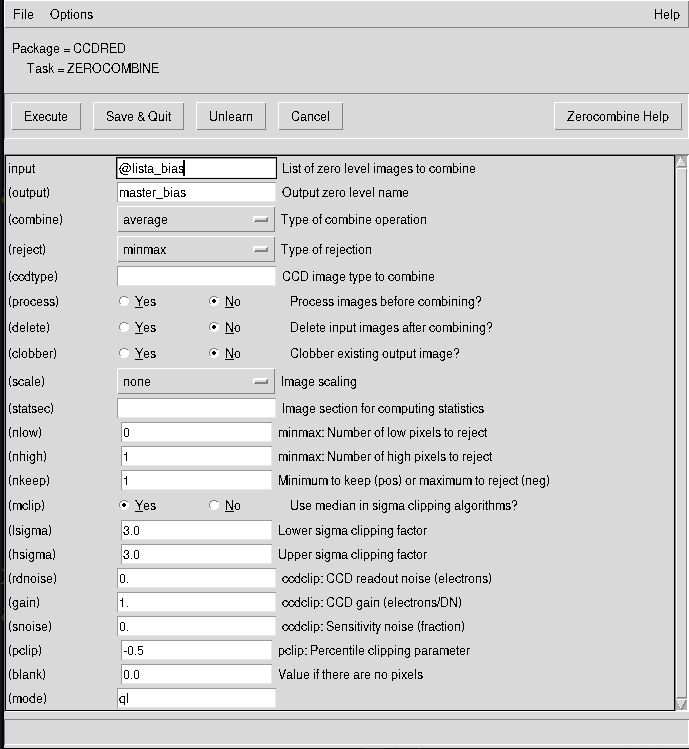
\includegraphics[width=0.7\textwidth]{figures/pyraf-zerocombine.png}
	\caption{Parámetros para combinar las imágenes de bias.}
	\label{fig:pyraf-zerocombine} 
\end{figure}

En el campo llamdo \pynorm{'input'} debes escribir el nombre de la lista que acabamos de crear. Para que esto funcione, el nombre de la lista debe tener al inicio el símbolo <<\norbash{@}>>, como se muestra en la Figura \ref{fig:pyraf-zerocombine}. En el campo \pynorm{'output'} puedes colocar cualquier nombre (sin espacios), en este caso, lo hemos llamado \pynorm{'master_bias'}. El campo \pynorm{'ccdtype'} debe quedar vacío, ya que los headers de los datos tomados con el instrumento OSIRIS no cuentan con esa información. Los demás campos pueden quedar con los parámetros predeterminados. 

Presiona el botón llamado <<\bashbold{Execute}>> para ejecutar la tarea. Esto puede tomar un poco de tiempo. Si todo sale bien, la terminal de pyraf no mostrará ningún error y se verá de la siguiente manera: 

\begin{shell}
--> epar zerocombine

Task zerocombine is running...

--> 
\end{shell}

Puedes verificar que se creó el archivo \pynorm{'master_bias.fits'} con el comando \norbash{ls}. 

\subsection{Creando un archivo master flat}
Ahora que hemos combinado las imágenes de bias, podemos corregir las imágenes flat y luego combinarlas con \norbash{flatcombine}. Los datos de OSIRIS no necesitan ser corregidos por corriente oscura, así que la calibración de imágenes es más sencilla para estos datos. Como se mencionó antes, a pesar de que las tareas son las mismas, cada proceso de calibración es distinto dependiendo de los instrumentos.

Para corregir las imágenes flat, primero dirijámonos a la carpeta donde están contenidas:

\begin{shell}
--> cd ../flat
--> pwd
/home/user/OB0001/flat
\end{shell}

Revisemos qué hay en la carpeta:

\begin{shell}
--> ls
0002615401-20200712-OSIRIS-OsirisSkyFlat1.fits
0002615420-20200712-OSIRIS-OsirisSkyFlat1.fits
0002615422-20200712-OSIRIS-OsirisSkyFlat1.fits
0002615450-20200712-OSIRIS-OsirisSkyFlat1.fits
0002615473-20200712-OSIRIS-OsirisSkyFlat1.fits
0002615484-20200712-OSIRIS-OsirisSkyFlat1.fits
0002615515-20200712-OSIRIS-OsirisSkyFlat1.fits
0002615546-20200712-OSIRIS-OsirisSkyFlat1.fits
0002615584-20200712-OSIRIS-OsirisSkyFlat1.fits
0002615608-20200712-OSIRIS-OsirisSkyFlat1.fits
-->
\end{shell}

De nuevo debemos crear un archivo de texto que contenga los nombres de todas las imágenes:
\begin{shell}
--> ls *.fits > lista_flat
--> 
\end{shell}
Además, debemos crear una segunda lista que contendrá los nombres de las imágenes flat corregidas por bias. La forma más fácil de hacerlo es editar el archivo que acabamos de crear y agregarle una palabra extra al final de cada elemento pero antes de la extensión \norbash{.fits} y luego guardarlo en la misma carpeta con un nuevo nombre. Podemos hacerlo con el editor \norbash{gedit} o con \norbash{geany}. Podemos guardar el nuevo archivo con el nombre \pynorm{'lista_flat_corredted'}, por ejemplo. 

Para ser claros, el contenido del archivo \pynorm{'lista_flat'} debe tener lo siguiente:

\begin{shell}
--> cat lista_flat
0002615401-20200712-OSIRIS-OsirisSkyFlat1.fits
0002615420-20200712-OSIRIS-OsirisSkyFlat1.fits
0002615422-20200712-OSIRIS-OsirisSkyFlat1.fits
0002615450-20200712-OSIRIS-OsirisSkyFlat1.fits
0002615473-20200712-OSIRIS-OsirisSkyFlat1.fits
0002615484-20200712-OSIRIS-OsirisSkyFlat1.fits
0002615515-20200712-OSIRIS-OsirisSkyFlat1.fits
0002615546-20200712-OSIRIS-OsirisSkyFlat1.fits
0002615584-20200712-OSIRIS-OsirisSkyFlat1.fits
0002615608-20200712-OSIRIS-OsirisSkyFlat1.fits
-->
\end{shell}

Mientras que el contenido del archivo \pynorm{'lista_flat_corrected'} debe verse así:

\begin{shell}
--> cat lista_flat_corrected
0002615401-20200712-OSIRIS-OsirisSkyFlat1_corrected.fits
0002615420-20200712-OSIRIS-OsirisSkyFlat1_corrected.fits
0002615422-20200712-OSIRIS-OsirisSkyFlat1_corrected.fits
0002615450-20200712-OSIRIS-OsirisSkyFlat1_corrected.fits
0002615473-20200712-OSIRIS-OsirisSkyFlat1_corrected.fits
0002615484-20200712-OSIRIS-OsirisSkyFlat1_corrected.fits
0002615515-20200712-OSIRIS-OsirisSkyFlat1_corrected.fits
0002615546-20200712-OSIRIS-OsirisSkyFlat1_corrected.fits
0002615584-20200712-OSIRIS-OsirisSkyFlat1_corrected.fits
0002615608-20200712-OSIRIS-OsirisSkyFlat1_corrected.fits
\end{shell}

Con estas dos listas podemos realizar la tarea llamada <<\norbash{ccdproc}>>. Vamos a editar sus parámetros para aplicar la corrección por bias:

\begin{shell}
--> epar ccdproc
\end{shell}

\begin{figure}[htb]
  \centering
	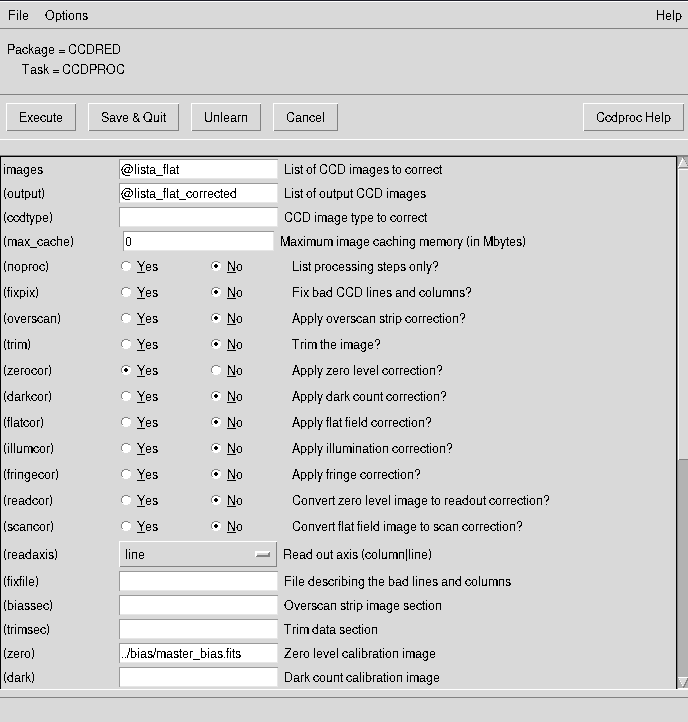
\includegraphics[width=0.7\textwidth]{figures/pyraf-correct-flat.png}
	\caption{Parámetros de la tarea \norbash{ccdproc}.}
	\label{fig:pyraf-correct-flat} 
\end{figure}

Los parámetros de la Figura \ref{fig:pyraf-correct-flat} que por el momento nos importan son \pynorm{'images'} donde debemos colocar la lista inicial de imágenes flat y a la que llamamos \pynorm{'lista_flat'}. En el parámetro \pynorm{'output'} colocaremos la segunda lista, llamada \pynorm{'lista_flat_corrected'}. El parámetro \pynorm{'ccdtype'} de nuevo quedará vacío y en todos los porcesos que involucren seleccionar \norbash{Yes/No}, dejaremos seleccionado en \norbash{Yes} únicamente al campo llamado \pynorm{'zerocor'}, cuya descripción es \pynorm{'Apply zero level correction?'}. Todos los demás deben seleccionarse en <<\norbash{No}>>. En el campo llamado \pynorm{'(zero)'} cuya descripción es \pynorm{'Zero level calibration image'}, debemos colocar la ruta hacia la imagen de master bias que creamos anteriormente. En este caso se colocó la ruta relativa, ya que nos encontramos dentro de la carpeta de flats. 

Si intentas ejecutar la tarea, se generará un error que dice que el tamaño de los DATASEC y CCDSEC no coinciden:
\begin{shell}
IrafError: Error running IRAF task ccdproc
IRAF task terminated abnormally
ERROR (1, "Size of DATASEC and CCDSEC do not agree")

--> 
\end{shell}

Esto es algo que ocurre con los datos de OSIRIS, para corregirlo, debemos editar los headers de las imágenes flat y del master bias con ayuda de la tarea <<\norbash{hedit}>>. Ejecuta dos veces el comando <<\norbash{epar hedit}>>. Una vez para editar el master bias y la otra para editar la lista de los flat iniciales. Coloca los parámetros tal como se muestra en la Figura \ref{fig:pyraf-hedit-flat}.

\begin{figure}[htb]
  \centering
	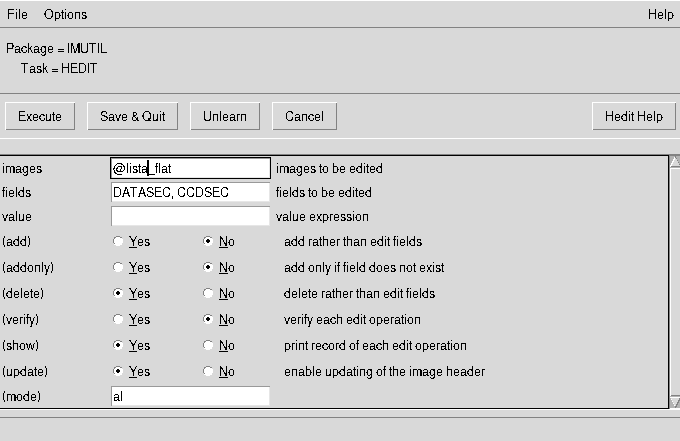
\includegraphics[width=0.48\textwidth]{figures/pyraf-hedit-flat.png}
	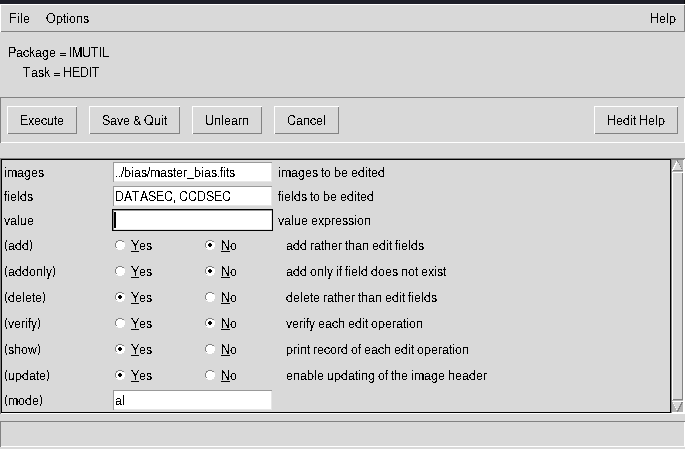
\includegraphics[width=0.48\textwidth]{figures/pyraf-hedit-master-bias.png}
	\caption{Parámetros para editar el header de las imágenes usando \norbash{hedit}.}
	\label{fig:pyraf-hedit-flat} 
\end{figure}

Ahora puedes volver a ejecutar el comando \norbash{ccdproc} y no se debería generar ningún error. Y editamos los parámetros de \norbash{ccdproc} anteriormente, así que no es necesario utilizar \norbash{epar ccdproc}. Basta con escribir \norbash{ccdproc} y presionar la tecla Enter para confirmar los parámetros de entrada:

\begin{shell}
--> ccdproc
List of CCD images to correct ('@lista_flat'): 


\end{shell}

La tarea puede tardar unos cuantos segundos. Cuando termine, puedes verificar con el comando \norbash{ls} que se crearon las imágenes cuyo nombre termina con \pynorm{'_corrected.fits'}. 

Usaremos esas imágenes que se acaban de crear para generar el archivo master flat. Para lograrlo, usamos el comando \norbash{epar flatcombine} que nos mostrará la interfaz para editar los parámetros:

\begin{shell}
--> epar flatcombine

\end{shell}

\begin{figure}[htb]
  \centering
	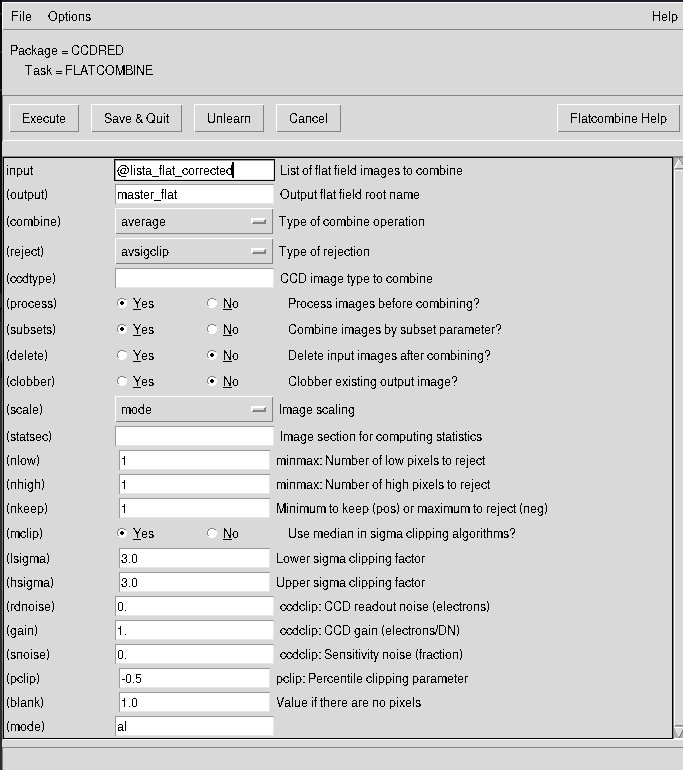
\includegraphics[width=0.7\textwidth]{figures/pyraf-flatcombine.png}
	\caption{Parámetros de la tarea \norbash{flatcombine}.}
	\label{fig:pyraf-flatcombine} 
\end{figure}

Coloca los parámetros tal como se muestran en la Figura \ref{fig:pyraf-flatcombine} y presiona el botón \bashbold{Execute}. Esto no debería generar nungún error pero sí podría tardar un tiempo en terminar. 

Puedes verificar que se creó un archivo llamado \pynorm{'master_flat.fits'} con ayuda del comando \norbash{ls}. En la siguiente clase usaremos los dos archivos, \pynorm{'master_bias.fits'} y \pynorm{'master_flat.fits'} para corregir las imágenes de objeto de este conjunto de datos. 

